\documentclass[11pt]{article}
\usepackage[margin=1in]{geometry}
\usepackage[T1]{fontenc}
\usepackage[utf8]{inputenc}
\usepackage{amsmath,amssymb,bm}
\usepackage{graphicx}
\usepackage[hidelinks]{hyperref}

\newcommand{\wt}{\widetilde}
\newcommand{\ket}[1]{|#1\rangle}
\newcommand{\bra}[1]{\langle #1|}
\newcommand{\one}{\mathbf{1}}

\title{A corrected pole picture for a shortcut into an absorbing site on a one-dimensional ring}
\author{}
\date{}

\begin{document}
\maketitle

\begin{abstract}
This note records the corrected stochastic interpretation of a shortcut from a
ring site into an absorbing target.  The key point is that, after the absorbing
site has been removed from the transient state space, the shortcut is a killing
channel rather than a probability-conserving transfer between transient sites.
This changes the sign in the rank-one resolvent denominator, invalidates the
old pole picture, and separates the asymptotic tail question from finite-time
visual bimodality.
\end{abstract}

\section{Role of this note}

This document has a different job from the in-place redline audit of Luca's
original manuscript.  The redline audit is author-facing: it preserves the
original text and marks the precise wrong steps.  This note is the cleaned
research-facing version.  It can sit inside the Valley-K ring material as the
corrected reference for the absorbing shortcut calculation.

For the broader one-dimensional ring programme, the calculation is useful in
three ways.  First, it gives a small exactly-checkable model in which shortcut
strength changes the first-passage tail.  Second, it provides a warning about
rank-one updates: a shortcut into an absorbing target is not algebraically the
same object as a shortcut into another live state.  Third, it gives a clean test
case for separating asymptotic tail decay from finite-time shape effects such as
apparent bimodality.

\section{Transient-space model}

Let the ring have \(N\) sites and let \(v\) be absorbing.  The transient state
space is the set of all sites except \(v\).  Let \(P_0\) be the transient
transition matrix for the lazy nearest-neighbour walk with absorbing target
already removed.  Suppose a shortcut starts at \(u\) and lands at \(v\).  If
\(\beta\) is the shortcut strength and \(q\) is the move probability, define
\[
  \lambda=\beta(1-q).
\]
Because the endpoint \(v\) is absorbing, the shortcut removes probability from
the transient state space.  Therefore the correct transient matrix is
\begin{equation}
  P_\beta=P_0-\lambda\ket{u}\bra{u}.
  \label{eq:killed-transient}
\end{equation}
This is the sign that the original pole diagram missed.

\section{Corrected rank-one resolvent}

Let
\[
  W(z)=(I-zP_0)^{-1}
\]
be the baseline transient resolvent.  The corrected shortcut resolvent is
\begin{equation}
  (I-zP_\beta)^{-1}
  =
  W(z)
  -
  \frac{z\lambda\, W(z)\ket{u}\bra{u}W(z)}
  {1+z\lambda W_{u,u}(z)}.
  \label{eq:corrected-resolvent}
\end{equation}
The plus sign in the denominator is forced by
\(P_\beta=P_0-\lambda\ket{u}\bra{u}\).  Any pole equation derived from
\[
  1-z\lambda W_{u,u}(z)
\]
belongs to the wrong probability-conserving shortcut model.  It should not be
used for the shortcut-to-absorbing-target calculation.

\section{Symmetric ring and pole geometry}

In the symmetric case let \(N=2L\), \(v=0\), and \(u=L\).  Write
\[
  s=\frac1z,
  \qquad
  y=\frac{s-1+q}{q},
  \qquad
  a=\frac{q}{\beta(1-q)}.
\]
The Chebyshev form of the corrected pole denominator can be written as
\begin{equation}
  D_+(s)=a+\Phi_L(s),
  \qquad
  \Phi_L(s)=T_L(y)U_{L-1}(y),
  \label{eq:corrected-pole-denominator}
\end{equation}
where \(T_L\) and \(U_{L-1}\) are Chebyshev polynomials of the first and second
kind.  Thus the corrected zero condition is
\begin{equation}
  \Phi_L(s)=-a.
  \label{eq:corrected-pole-condition}
\end{equation}
The old sign instead asks for \(\Phi_L(s)=+a\).  That is the wrong pole
geometry for the stochastic shortcut-to-absorbing-target interpretation.

\begin{figure}[t]
  \centering
  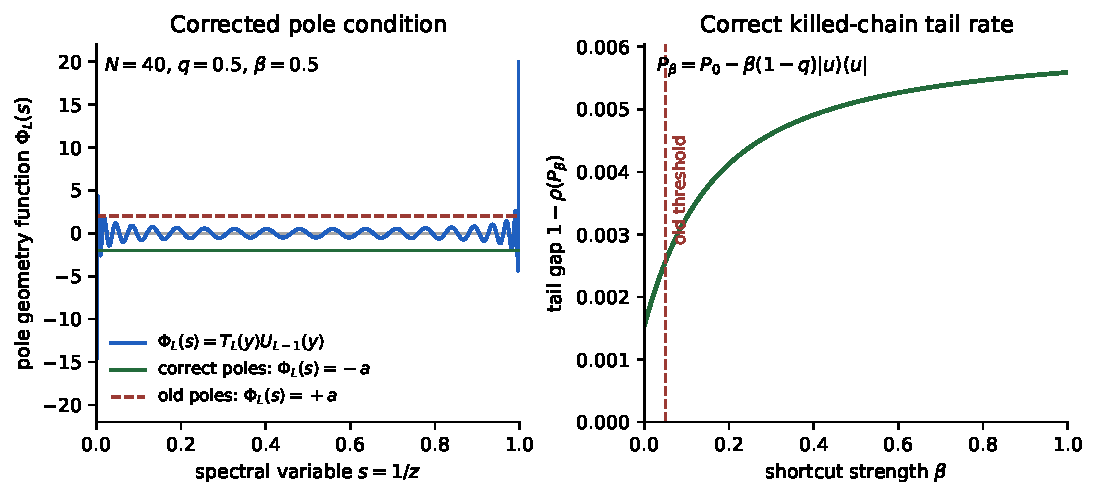
\includegraphics[width=\linewidth]{figures/corrected_pole_geometry.pdf}
  \caption{Corrected pole geometry and tail-rate diagnostic for the symmetric
  absorbing shortcut on a ring.  Left: the corrected pole equation uses
  \(\Phi_L(s)=-a\), whereas the old manuscript used the opposite sign.  Right:
  the tail gap \(1-\rho(P_\beta)\), computed directly from the killed transient
  matrix in \eqref{eq:killed-transient}, varies smoothly with shortcut strength;
  the old threshold is shown only as a marker for the invalid sign-based
  criterion.}
  \label{fig:corrected-pole-geometry}
\end{figure}

\section{Tail asymptotics and finite-time shape}

The first-passage tail is controlled by the spectral radius of the killed
transient matrix \(P_\beta\), or equivalently by the corrected pole of the
generating function with largest modulus in \(z\).  In \(s=1/z\) variables this
dominant value is the largest relevant decay factor below one.  The tail has the
form
\[
  \Pr(T=t) \sim C\,\rho(P_\beta)^{t-1}
\]
for the appropriate residue \(C\), provided the dominant pole is simple.

This is not the same question as finite-time visual bimodality.  A distribution
can have two visible finite-time scales while still having a single asymptotic
tail.  Conversely, a change in the corrected tail gap does not by itself prove a
visual bimodality threshold.  Finite-time bimodality should be checked from the
full coefficient sequence or by direct simulation of the killed chain.

\section{Implication for the Valley-K ring work}

This corrected note should be treated as a local analytic guardrail for the
one-dimensional ring part of the Valley-K project.  It says exactly which
shortcut perturbation is being studied, supplies the corrected pole equation,
and gives a reproducible figure based on the same killed-chain model.  The note
is most useful as a technical appendix or companion to numerical experiments:
it can calibrate simulations, check finite-time first-passage plots, and prevent
the invalid threshold from being used as an explanation of ring bimodality.

\end{document}
